\documentclass{beamer}
%
% Choose how your presentation looks.
%
% For more themes, color themes and font themes, see:
% http://deic.uab.es/~iblanes/beamer_gallery/index_by_theme.html
%
\mode<presentation>
{
	\usetheme{Madrid}
  %\usetheme{default}      % or try Darmstadt, Madrid, Warsaw, ...
  \usecolortheme{default} % or try albatross, beaver, crane, ...
  \usefonttheme{default}  % or try serif, structurebold, ...
  \setbeamertemplate{navigation symbols}{}
  \setbeamertemplate{caption}[numbered]
} 

\usepackage[english]{babel}
\usepackage[utf8x]{inputenc}
\usepackage{textcomp}
\usepackage{caption}
\usepackage[bottom]{footmisc}


\title[Final Seminar]{On the list coloring of 1-band buffering graphs}
\author{Marine Collery, Benjamin Martin Seregi}
\institute{KTH Royal Institute of Technology\\
II2202, Fall 2017, Period 1-2}
\date{12/01/2018}

\begin{document}

\begin{frame}
  \titlepage
\end{frame}

% Uncomment these lines for an automatically generated outline.
%\begin{frame}{Outline}
%  \tableofcontents
%\end{frame}
%------------------------------------------------
\section{Introduction}

\begin{frame}{Problem Statement}

TO BE COMPLETED

\end{frame}

%------------------------------------------------
\section{Background}

\begin{frame}{Background and related work}

TO BE COMPLETED

\end{frame}

%------------------------------------------------
\section{Method used to solve the problem}

\begin{frame}{Method used to solve the problem}

\begin{itemize}
  \item \textbf{analytical} method
  \item 1-band buffering cellular topology \textrightarrow{} easily modeled as a graph.
  \item Prove solution = optimal and fast\\
  \textrightarrow{} empirical methods : impossible 
  would not cover all the possible topologies that might arise in network deployments
\end{itemize}

\vskip 1cm

Testing:
\begin{itemize}
  \item Generate graphs \& coloration
  \item Create database
  \item Analyze
\end{itemize}

\end{frame}


%------------------------------------------------
\section{Results and Analysis}

\begin{frame}{Results and Analysis}

\small{\textit{Implementation based on JGraphT [1] libraries}}

\begin{block}{}

\begin{enumerate}
  \item Generate a \textbf{Cellular} Graph
  \item Construct an \textbf{Acyclic 3-bounded} orientation of a Cellular Graph
  \item Find the \textbf{Kernel} in a Directed Acyclic Graph
\end{enumerate}

\end{block}

\textrightarrow{}  Generation of Colored Cellular Graphs

\begin{figure}
\centering
\begin{minipage}{.5\textwidth}
  \centering
  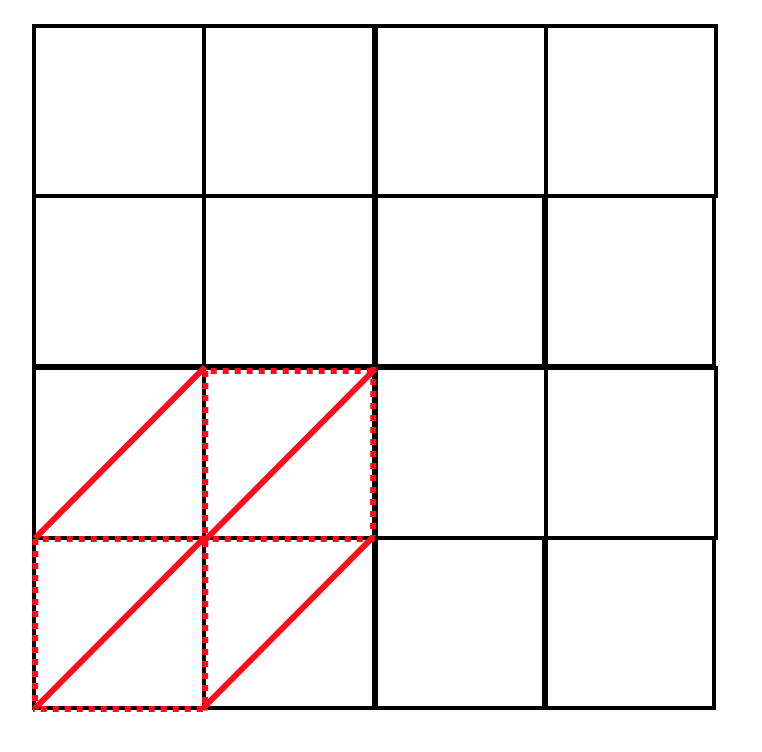
\includegraphics[width=0.5\linewidth]{cellGeneration.png}
  \caption{Cellular Graph generated from Grid}
\end{minipage}%
\begin{minipage}{.5\textwidth}
  \centering
  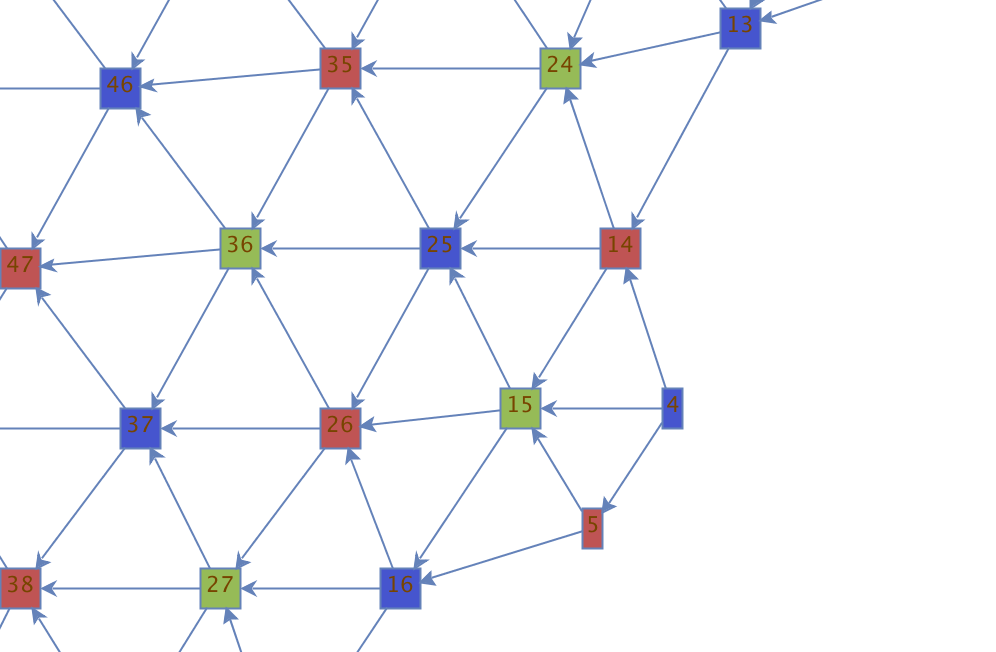
\includegraphics[width=0.65\linewidth]{3colors.png}
  \caption{Part of a colored Cellular Graph}
\end{minipage}
\end{figure}

\scriptsize [1]“Welcome to JGraphT - a free Java Graph Library.” [Online]. Available: http://jgrapht.org/.
\end{frame}



%------------------------------------------------
\begin{frame}{Results and Analysis}

\begin{block}{Running Time Comparison with ILP Solution from GNU}
2 Parameters to evaluate for the time consumption:
\begin{itemize}
\item \textbf{Size} of the Graph
\item \textbf{Nbr of Colors} Available
\end{itemize}
 
\end{block}

Generation of numerous amount of data \textrightarrow{} Space \& Time limit\\
\textrightarrow{}  Bash Scripts to \textbf{generate}, \textbf{verify}, \textbf{compare} and \textbf{save}\\
\textrightarrow{}  Analysis of the quantitative data in R Studio

% \begin{figure}
% 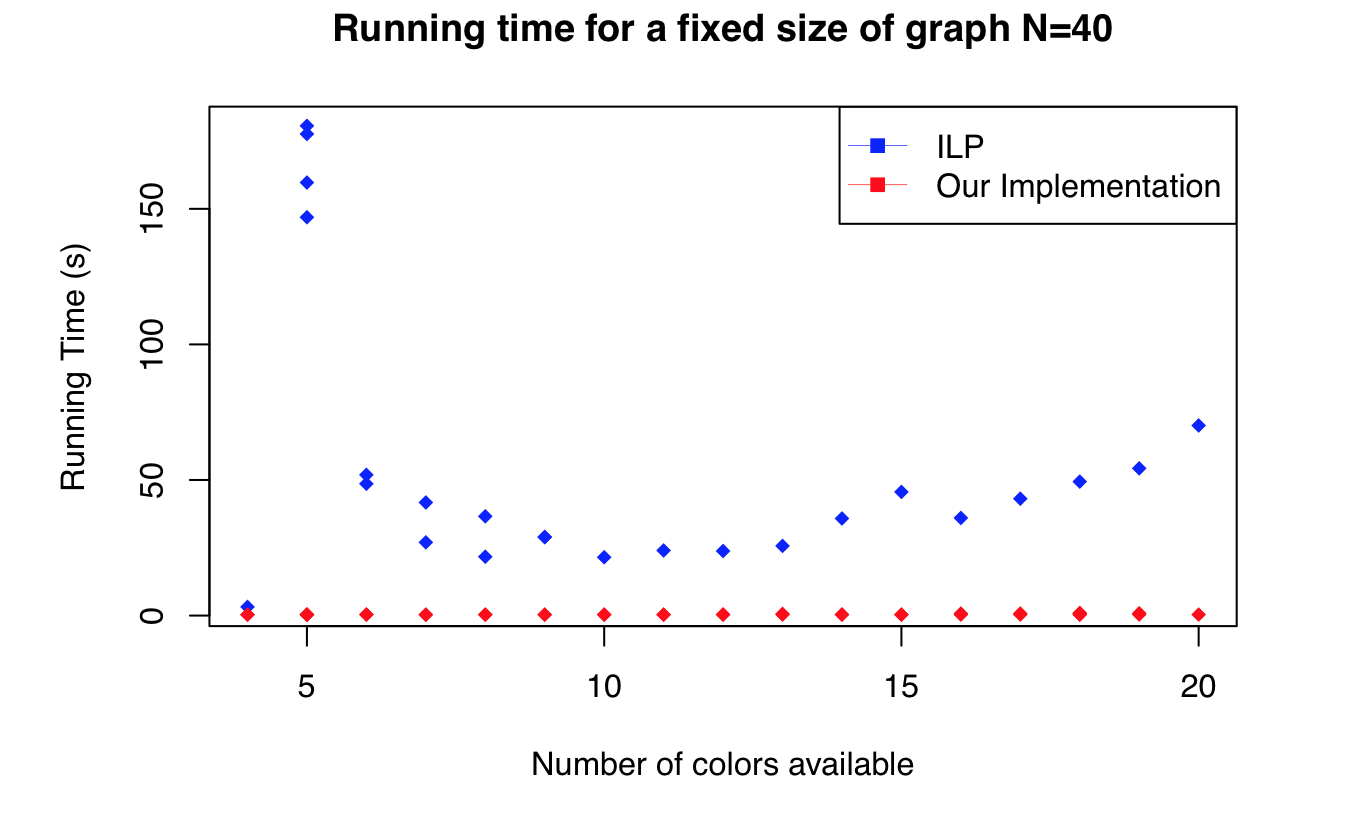
\includegraphics[width=0.8\linewidth]{40SizeRunTime.png}
% \end{figure}

\begin{figure}
\centering
\begin{minipage}{.5\textwidth}
  \centering
  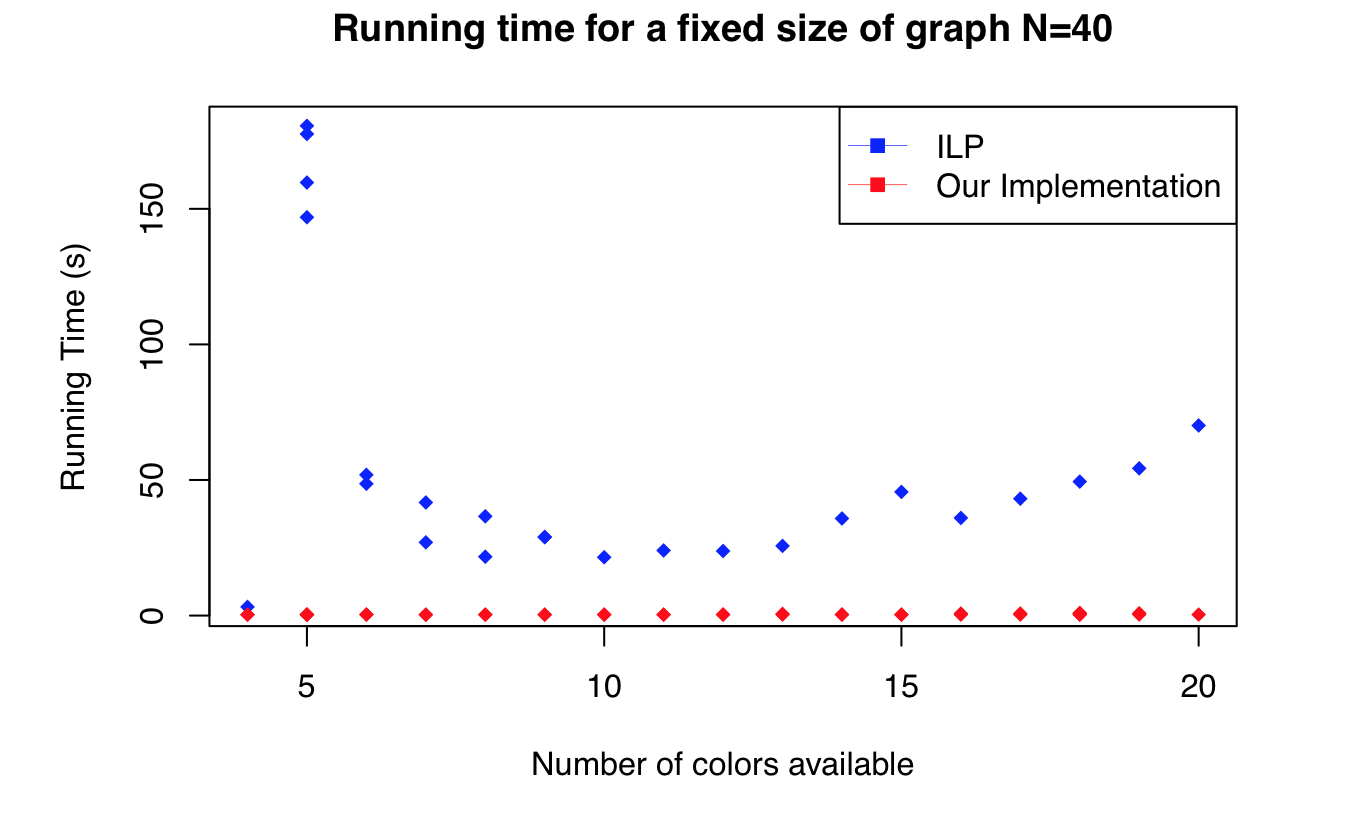
\includegraphics[width=1\linewidth]{40SizeRunTime.png}
  \label{fig:test1}
\end{minipage}%
\begin{minipage}{.5\textwidth}
  \centering
  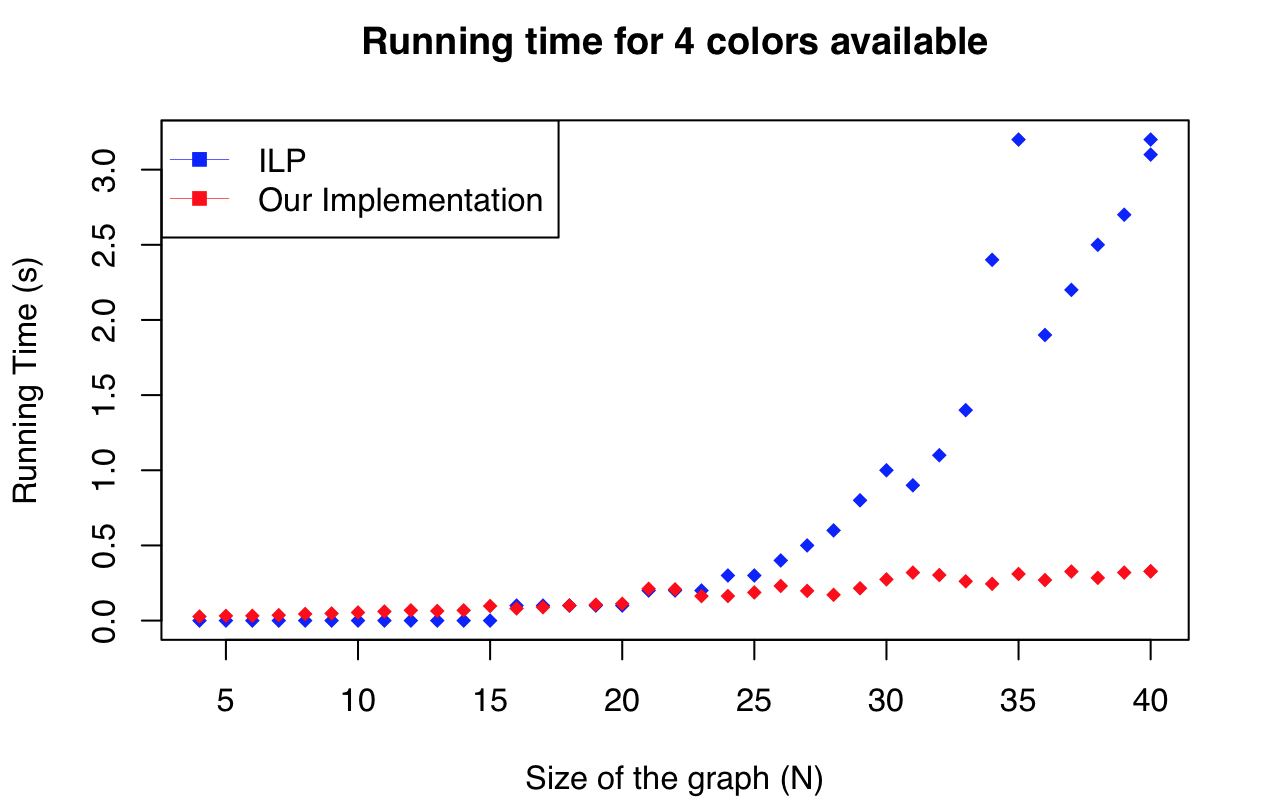
\includegraphics[width=1\linewidth]{4colorsRunTime.png}
  \label{fig:test2}
\end{minipage}
\end{figure}

\vskip 1cm

\end{frame}

%------------------------------------------------
\section{Conclusion}

\begin{frame}{Conclusion}

\begin{block}{}
\begin{itemize}
\item Cellular graph are \textbf{4-choosable} \textrightarrow{} tested
\item When 4 colors available for all Nodes \textrightarrow{} \textbf{3} colors used\\
\textrightarrow{} 1-band buffering cellular graphs are \textbf{3-colorable}
\end{itemize}
 
\end{block}
\vskip 1cm
\begin{block}{}

\begin{itemize}
\item Running Time (Size, Nbr Available Colors)
\item More \textbf{efficient} than ILP implementation (+ large graph)
\end{itemize}

\end{block}

\end{frame}


%------------------------------------------------
\section{Future Work}

\begin{frame}{Future Work}

\begin{itemize}
  \item Your introduction goes here!
  \item Use \texttt{itemize} to organize your main points.
\end{itemize}

\vskip 1cm

\begin{block}{Examples}
Some examples of commonly used commands and features are included, to help you get started.
\end{block}

\end{frame}

%------------------------------------------------
\section{Questions}

\begin{frame}
\Huge{Thank you for your attention !\\
Do you have any questions?}
\end{frame}




\end{document}
